\subsection{Conceptual Model} \label{ConsMod}
\Cref{ConceptualModelPicture} shows a conceptual model between different domains of requirements and actions. this conceptual model is created to give an overview of what has been defined in the rest of \nameref{DesDev} in \cref{DesDev}. The four boxes with sharp corners are seen as domains, where the boxes with soft corners are requirements to the different domains, the arrows with text are actions that sets new requirements.

\begin{figure}[H]
	\centering
    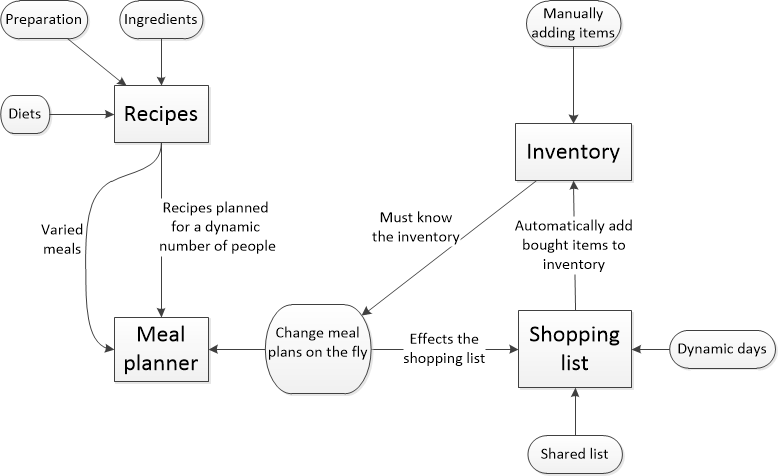
\includegraphics[width=1\textwidth]{Grafik/conceptualModel}
	\caption{Conceptual Model}
	\label{ConceptualModelPicture}
\end{figure}